\documentclass{optica-article}

\journal{opticajournal} % for journals or Optica Open

\articletype{Research Article}

\usepackage{lineno}
\usepackage{soul}
\usepackage{booktabs}
\linenumbers % Turn off line numbering for Optica Open preprint submissions.

\begin{document}

\title{From Fog Chamber to Aircraft Window: Joint Training on Pixel-Registered and Synthetic Fog for Cross-Domain Defogging}

\author{Alexander Ingold,\authormark{1} Sabina D. Menon,\authormark{2} Manya Yellepeddy,\authormark{2} Alec Ikei,\authormark{2} John D. Hodges,\authormark{2} Jordan Baker,\authormark{2} Syed N. Qadri,\authormark{2} and Rajesh Menon\authormark{1,*}}

\address{\authormark{1} Department of Electrical and Computer Engineering, University of Utah, Salt Lake City, UT 84112, USA\\
\authormark{2} U.S. Naval Research Laboratory Remote Sensing Division, Washington DC 20375, USA.\\}

\email{\authormark{*}rmenon@eng.utah.edu} %% email address is required; see note below about the corresponding author designation

% use {asbstract*} to suppress the copyright line. Copyright information will be added in production

\begin{abstract*}
We present a defogging pipeline trained from random initialization on
a deterministic mixture of controlled fog-chamber pairs and
domain-randomized synthetic outdoor fog. The two sources are
interleaved throughout optimization rather than used as pretraining
and fine-tuning stages. The primary schedule contains 247{,}150
chamber updates and 2{,}600 synthetic updates (1.04\% of all
updates), matching the predetermined synthetic-update budget while
distributing that exposure across chamber training. A single-camera fog imager
photographs a flat-panel display through an artificial-fog enclosure
with a fixed 114~mm scattering path, producing 5{,}495
pixel-registered foggy/clear pairs. Exact registration supports
pixelwise reconstruction training and a paired Laplacian ratio that
predicts per-image restoration quality better than single-image
proxies (Spearman $\rho=0.632$ versus $0.399$). A uniform comparison
of 30 restoration backbones on the chamber data places NAFNet first
(24.33~dB~/~0.7912~SSIM), with a compact alternative within
1.29~dB at 3\% of the parameter count. Using NAFNet, joint mixed-data
training reaches 24.41~dB~/~0.7936~SSIM on the same 552-image chamber
holdout, while the synthetic component is included to target
oversaturation and tiled-inference artifacts during transfer. The
mixed model is applied without target-domain training to
chamber-free fog and iPhone video recorded through an aircraft
window, providing tests across unseen scenes, optics, and sensors.
A ResNet-50 check shows that chamber restoration preserves
semantic content, and separate paired adaptation reaches
20.71~dB~/~0.683~SSIM on a non-overlapping O-HAZE/NH-HAZE split.
These results show how optically controlled paired data and a small,
concurrent synthetic component can be used together without making
synthetic-benchmark performance the optimization target.
\end{abstract*}

%% ============================================================
\section{Introduction}
\label{sec:intro}
%% ============================================================
 
Fog and haze attenuate scene radiance along the line of sight and
add scattered ambient light, reducing contrast and suppressing fine
detail. The standard atmospheric scattering model expresses an
observed pixel as a convex mixture of the attenuated scene radiance
and the airlight, weighted by a transmission term that decays with
optical depth \cite{koschmieder1924,narasimhan2002vision}.
Recovering a clear image from a single foggy observation is
therefore underconstrained: scene radiance, airlight, and
depth-dependent transmission are all unknown from one measurement
per pixel \cite{narasimhan2002vision}.
\begin{figure}[htbp]
\centering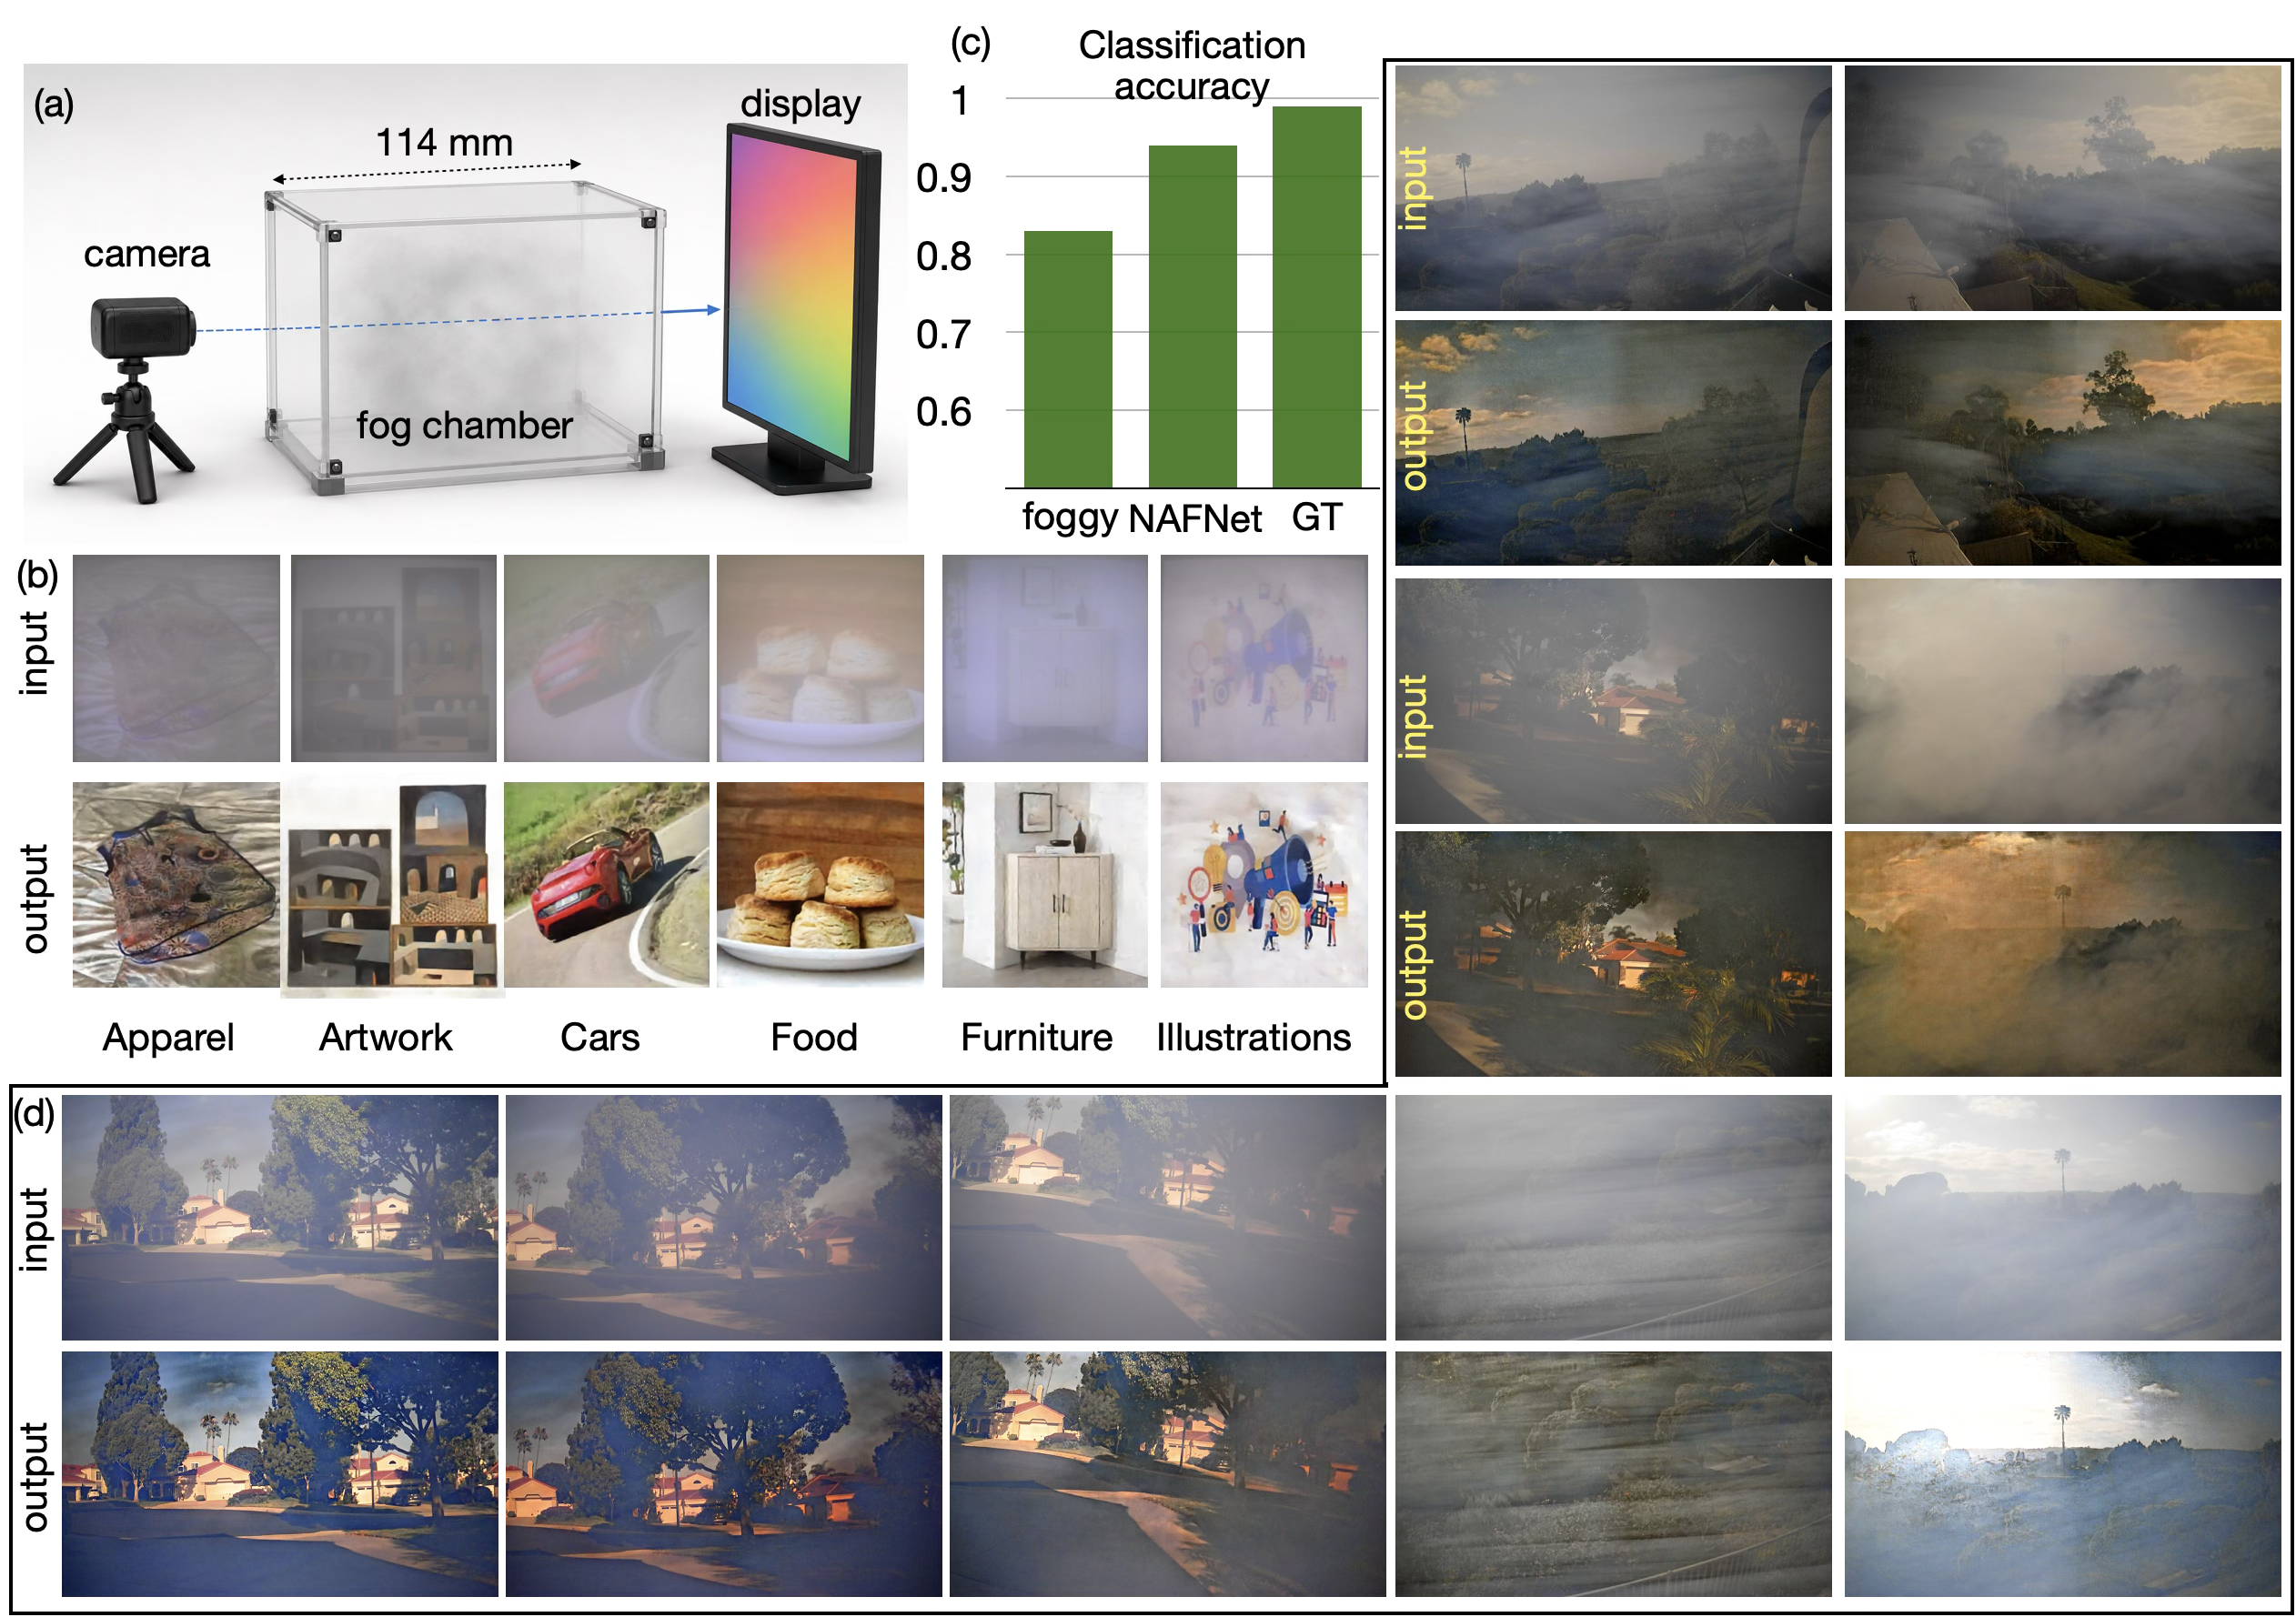
\includegraphics[width=\linewidth]{fog_chamber_overview.png}
\caption{Controlled fog-chamber training, benchmark results, and
a chamber-only transfer check. (a)~Pipeline overview: foggy
images are captured through a fog chamber with a fixed 114~mm
scattering path, and the pixel-registered ground-truth images are
used to train a deep restoration network with pixel-exact $L_1$
supervision. (b)~Representative test-set results across the six
content categories (top row: foggy input; bottom row: NAFNet
prediction); on the 552-image held-out split NAFNet attains mean
PSNR / SSIM of 24.33~dB~/~0.7912. (c)~Category-classification
accuracy of a ResNet-50 evaluated on foggy inputs, NAFNet-defogged
outputs, and ground-truth images, quantifying how much
semantic content the restoration recovers relative to fog
degradation. (d)~Transfer to chamber-free fog generated by the fog
machine placed directly in front of the camera, producing
spatially nonuniform, time-varying scattering across a range of
outdoor scenes (top row: foggy input; bottom row: output from the
chamber-benchmark NAFNet). Together, panels~(b)--(d) show that the
chamber-only model
restores both pixel-level structure and semantic content under
controlled fog and continues to remove the bulk of the scattering
when the fog dynamics depart from the chamber regime. Mixed-model
chamber-free results are reported separately in the Supplement.}
\label{fig:fog_chamber_overview}
\end{figure}

\subsection{Prior-based and learned restoration}
 
Early methods made the inverse problem tractable with statistical
priors on outdoor scenes, notably the dark channel prior
\cite{he2010single} and the color attenuation prior
\cite{zhu2014single}. These priors are interpretable but fail for
bright or white content, unusual materials, and dense or
spatially uniform fog, and have no mechanism for non-natural
capture geometries. Deep learning shifted the field toward learned
restoration: DehazeNet \cite{cai2016dehazenet} and AOD-Net
\cite{li2017aod} estimated or embedded the scattering model;
GridDehazeNet \cite{liu2019griddehazenet}, FFA-Net
\cite{qin2020ffa}, and DehazeFormer \cite{song2023dehazeformer}
added multi-scale and attention mechanisms; and general-purpose
backbones such as NAFNet \cite{chen2022simple} showed that
streamlined direct-reconstruction networks rival more complex
designs. Surveys nevertheless emphasize a persistent gap between
synthetic-benchmark and real-haze performance
\cite{gui2021comprehensive}, and no large, uniformly trained
benchmark of modern backbones exists for an optically controlled,
exactly paired fog dataset. Paired calibration has also enabled
real-time reconstruction through dynamic scattering media
\cite{liu2024dynamic_scattering}, distinct from our passive
single-image fog-removal setting.
 
\subsection{Real-world paired data and the transfer problem}
 
Because aligned foggy/clear pairs are hard to acquire outdoors, the
field has relied on synthetic data, from SYNTHIA
\cite{ros2016synthia} and Foggy Cityscapes
\cite{sakaridis2018semantic} to curriculum adaptation
\cite{sakaridis2018model}. A central limitation is that synthetic training can fail when the generated fog distribution is too narrow or does not match real imaging conditions, and unpaired adversarial translation \cite{isola2017pix2pix,zhu2017unpaired} introduces hallucination
risk when faithful reconstruction matters. Real paired benchmarks
such as O-HAZE \cite{ancuti2018ohaze} and NH-HAZE
\cite{ancuti2020nhhaze} anchor the NTIRE challenges
\cite{ancuti2021ntire,histofusionnet2026} but contain only tens of
scenes, and recent methods continue to push real-image dehazing
\cite{chen2024pttd,chen2025dehazexl}.
 
Most directly relevant to the present work, Pollak and Menon
introduced Stereofog, a 10{,}067-pair real-world binocular dataset,
and demonstrated effective \texttt{pix2pix} defogging even under
dense fog \cite{pollak2024stereofog}. That study reached two
conclusions that motivate this paper. First, models trained on
generic synthetic fog failed on real images. Second, and more
fundamentally, the learned models transferred poorly to different
cameras and scenes without retraining, which the authors attributed
to adaptation to specific recording hardware. The binocular design
also captures the two views with separate cameras, introducing
residual misregistration that required shift-robust metrics and
favored adversarial translation, whose hallucination tendency the
authors flagged as a limitation. Whether a controlled, exactly
registered capture system combined with a small concurrent source
of randomized synthetic outdoor fog can instead produce models that
transfer across hardware and scenes has remained open.
 
\subsection{Gaps and contributions}
\label{sec:contributions}

The prior literature leaves three gaps: no optically controlled,
exactly paired fog dataset large enough for a uniform many-model
benchmark; little use of paired data to characterize the fog
itself; and few tests of cross-domain generalization from a
controlled imager to a completely different consumer sensor and
scene, let alone to motion video. We address these with an
end-to-end study centered on complementary paired data sources, a
paired difficulty metric, and a domain-randomized synthetic
generator; we deliberately use existing
restoration backbones rather than introducing a new architecture,
so the study focuses on the data and training regime rather than a
new model design. Our
contributions are:

\begin{enumerate}

\item \textbf{Joint mixed-data training.} The final NAFNet is trained
from random initialization by deterministically interleaving
247{,}150 chamber updates with 2{,}600 Mapillary synthetic-fog
updates. Synthetic updates therefore comprise 1.04\% of optimization
and are distributed across training rather than appended as a
separate fine-tuning stage. Light-fog measurements set only loose
generator ranges; the synthetic generator randomizes fog strength,
airlight, spatial variation, contrast, color, and noise.

\item \textbf{Cross-domain transfer checks across a graded
out-of-distribution sequence, including aircraft-window iPhone
video.} The mixed model is applied without target-domain training to
(i)~free-flowing fog generated outside the chamber by a fog machine placed
in front of the camera, in which the optical depth along the line of
sight is no longer fixed by chamber geometry, and (ii)~iPhone video captured
through an aircraft cabin window in flight
(Fig.~\ref{fig:aircraft}; Supplementary Videos~1 and~2). This
provides a direct test relevant to the cross-hardware transfer
limitation reported for real-world binocular
defogging~\cite{pollak2024stereofog}.

\item \textbf{A controlled, exactly registered fog imager and a
5{,}495-pair dataset.} A display-based imager photographs a flat-panel display through an artificial-fog enclosure
with a fixed 114~mm scattering path. Unlike binocular
capture~\cite{pollak2024stereofog}, single-camera display imaging
gives exact pixel registration, which both removes the need for
shift-robust metrics and enables direct reconstruction training
that avoids adversarial hallucination.

\item \textbf{A paired fog-difficulty metric.} The mean-absolute
Laplacian ratio, a paired refinement of the single-image Laplacian
variance used to grade fog density in prior
work~\cite{pollak2024stereofog}, predicts per-image restoration
quality with Spearman $\rho = 0.632$ (category-centered $0.590$),
far exceeding the best single-image proxy ($\rho = 0.399$).

\item \textbf{A 30-model benchmark with a semantic-content check.}
Thirty restoration backbones are trained under identical conditions
on the fog-chamber dataset, establishing a reproducible baseline
across contemporary defogging architectures and generic
image-to-image models. NAFNet~\cite{chen2022simple} ranks highest
(24.33~dB~/~0.7912~SSIM), while SpecAT~S2~\cite{yao2024specat} is
within 1.29~dB at 3\% of the parameter count. A ResNet-50
classifier evaluated on foggy, defogged, and clear inputs shows
that classification is already feasible directly from foggy
images, and that NAFNet defogging closes most of the residual gap
to ground truth (Fig.~\ref{fig:fog_chamber_overview}c), indicating
that the restoration preserves semantic content rather than only
low-level appearance.

\end{enumerate}
 
The dataset is public, and the code, simulator, trained models, and
demonstration videos will be released with the reproducibility
package. Section~2 describes the chamber geometry and paired metric,
Section~3 the methods, Section~4 the results, Section~5 the
discussion, and Section~6 concludes. The supplement provides split audits, metric definitions, the full benchmark table, classification and dark-channel-prior checks, simulator details, public real-haze protocols, fog-density statistics, and paired structure-loss analysis.

%% ============================================================
\section{Chamber geometry and paired metric}
\label{sec:fogphysics}
%% ============================================================
 
\subsection{Scattering model background and chamber geometry}
 
The atmospheric scattering model \cite{narasimhan2002vision} writes
the observed pixel as
 
\begin{equation}
  \mathbf{I}(\mathbf{x}) =
    \mathbf{J}(\mathbf{x})\,T(\mathbf{x})
    + \mathbf{A}\bigl[1 - T(\mathbf{x})\bigr],
  \qquad
  T(\mathbf{x}) = e^{-\beta\, d(\mathbf{x})},
  \label{eq:scattering}
\end{equation}
 
\noindent where $\mathbf{J}$ is the clear radiance, $\mathbf{A}$ the
global airlight, $T$ the transmission, $\beta$ the extinction
coefficient, and $d$ the path length. For the fog imager $d$ is
fixed by the chamber geometry. We use this model as a physical motivation for the synthetic fog simulator, not as a radiometric inversion of the fog-chamber data. The display, camera response, exposure and fog radiance were not independently calibrated, so we do not estimate a physical transmission map or extinction coefficient from the image pairs. The acrylic fog chamber had a 114~mm fog path length and 133 $\times$ 114~mm transverse dimensions (see Fig.~\ref{fig:fog_chamber_overview}). Artificial
fog was generated by an Eliminator Lighting VF400-E theatrical fog
machine using propylene-glycol fluid.
 
\subsection{A paired fog-difficulty metric}
\label{subsec:fogdifficulty}
 
Prior real-world work graded image-level fog severity by the variance of the
Laplacian of the foggy image alone \cite{pollak2024stereofog}.
Exact registration lets us instead form a \emph{paired}
high-frequency retention ratio,
 
\begin{equation}
  R_{\nabla^2} =
    \frac{\mathrm{mean}\!\left(|\nabla^2 \mathbf{I}_{\mathrm{fog}}|\right)}
         {\mathrm{mean}\!\left(|\nabla^2 \mathbf{I}_{\mathrm{clear}}|\right)},
  \label{eq:laplacian_ratio}
\end{equation}
 
\noindent which measures how much of the clear image's local
high-frequency structure survives the fog and normalizes out scene
content. On the 552-image split, $R_{\nabla^2}$ at one-pixel scale
predicts per-image NAFNet PSNR with Spearman $\rho = 0.632$
(category-centered $0.590$), substantially better than the best
single-image proxy (dark-channel 90th percentile, $\rho = 0.399$;
category-centered $0.312$). Supplementary Fig.~S6 summarizes the metric ranking, per-image relationship to NAFNet PSNR, and a representative paired Laplacian example. The full-metric search is in Supplementary Section~S10 and the image-domain power-spectral-density (PSD) analysis is in Supplementary Section~S9. The PSD analysis shows that high-frequency power retention was 8.9$\times$ lower than low-frequency retention in paired fog/clear images. 
 
%% ============================================================
\section{Methods}
\label{sec:methods}
%% ============================================================

Figure~\ref{fig:transfer_workflow} summarizes architecture selection
on the fog-chamber benchmark, joint mixed-data training, and the
separate task-specific public-haze checks.

\begin{figure}[htbp]
\centering
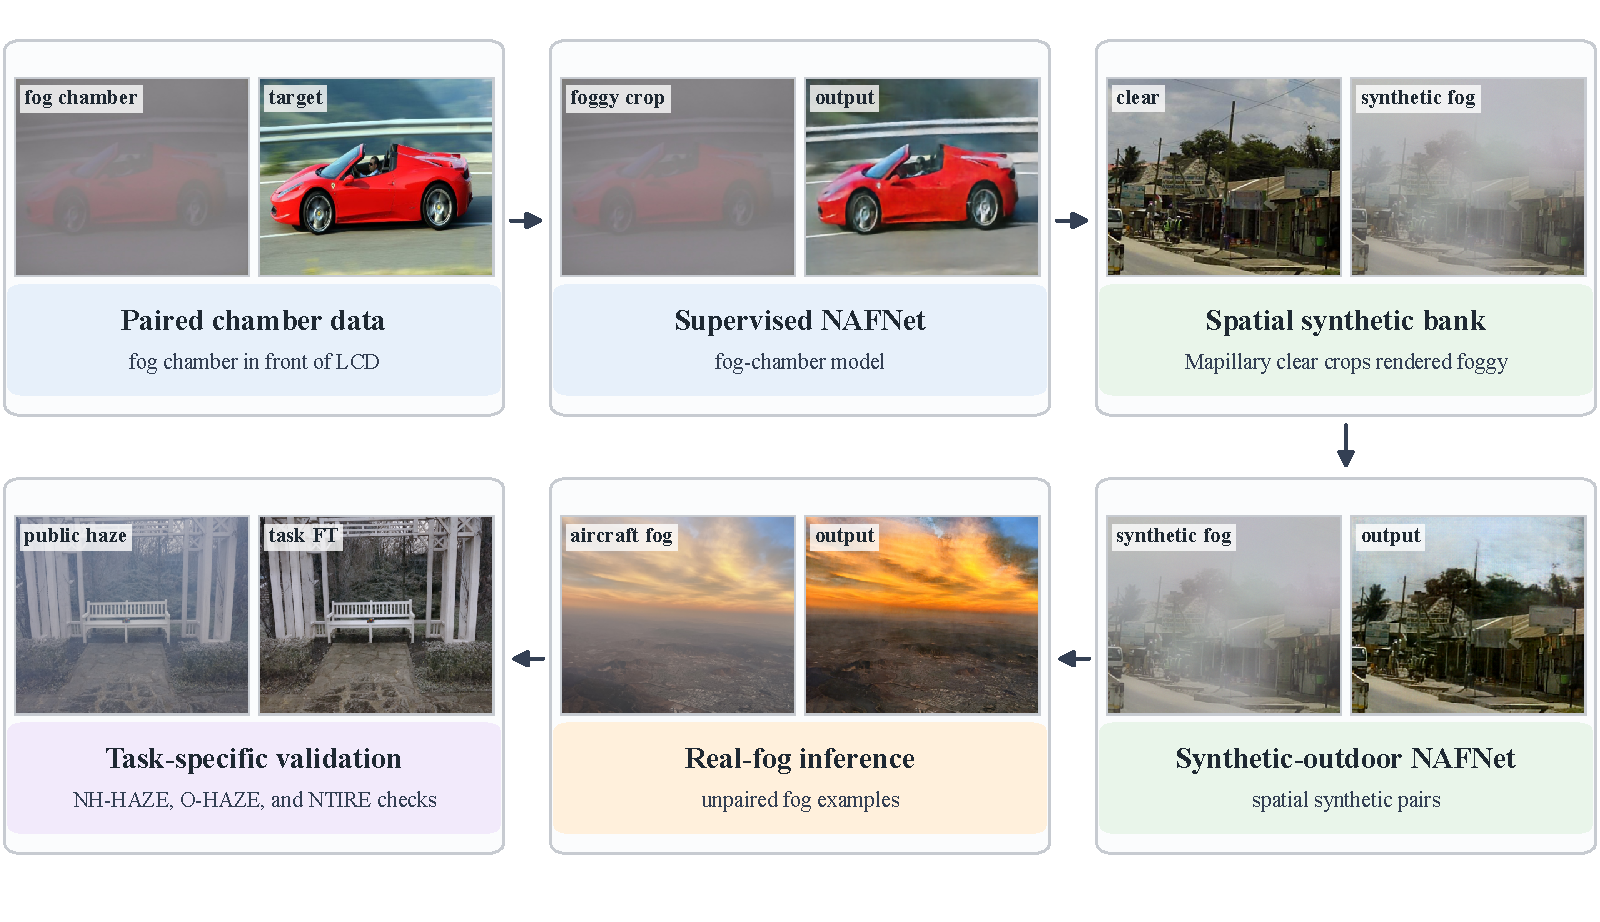
\includegraphics[width=\linewidth]{fig_transfer_workflow_schematic.pdf}
\caption{Mixed-data training and evaluation workflow. The
fog-chamber benchmark selects NAFNet as the restoration backbone.
The primary mixed-data model is then initialized randomly and trained
with chamber and synthetic Mapillary updates interleaved throughout
one optimization schedule; it is not initialized from the chamber
checkpoint. The mixed model is applied without target-domain
training to chamber-free, aircraft-window, and paired public-haze
examples. Separate NAFNet models provide supervised task-specific
O-HAZE/NH-HAZE and NTIRE checks.}
\label{fig:transfer_workflow}
\end{figure}
 
\subsection{Apparatus and dataset}
\label{subsec:apparatus}
 
As illustrated in Fig.~\ref{fig:fog_chamber_overview}(a), a flat-panel LCD presents the ground-truth target through an acrylic
enclosure of internal path length $114~\mathrm{mm}$ and transverse
cross-section $133 \times 114~\mathrm{mm}$, with fog from the VF400-E
machine; in some runs a vertical linear polarizer was placed before
the camera (noted where used). Single-camera display imaging yields
exact pixel registration without post-hoc alignment, in contrast to
binocular capture \cite{pollak2024stereofog}, and lets us train with
pixel-exact L1 reconstruction rather than adversarial losses (Fig.~\ref{fig:fog_chamber_overview}a).
Ground-truth images are drawn from a public $130\mathrm{k}$-image
archive at $512 \times 512$ across six categories \cite{singh130kimages}.
A deterministic every-tenth split yields 4{,}943 training and 552
held-out pairs (92 per category; 5{,}495 total). Full dataset roles
and split audits are in Supplementary Section~S1.
 
\subsection{Benchmark, classification, simulator, and mixed-data training}
\label{sec:methods-benchmark}
We trained thirty restoration backbones from random initialization on
the fog-chamber training split under identical conditions. No pretrained
restoration weights were loaded. Training used pixel-exact $L_1$ loss, Adam
optimizer~\cite{kingma2015adam}, learning rate $10^{-4}$, 50 epochs,
and $512\times512$ inputs (memory-heavy models used crops at the
same resolution). Each model was evaluated on the 552-image held-out
split by mean MAE, MSE, PSNR, and SSIM~\cite{wang2004ssim}, with
LPIPS~\cite{zhang2018lpips} additionally reported for the top five.
NAFNet~\cite{chen2022simple} ranked highest and was selected as the
backbone for the final mixed-data model and the separate
task-specific adaptation checks.

To assess whether restoration preserves semantic content rather than
merely pixel-level structure, we trained a ResNet-50
classifier~\cite{he2016deep} on five dataset categories excluding illustrations and
evaluated it on clear, foggy, and NAFNet-defogged images
(Fig.~\ref{fig:fog_chamber_overview}c). Classification from foggy
inputs already retains most of the ground-truth accuracy, and
NAFNet-defogged inputs close most of the remaining gap, indicating
that the restoration recovers semantically discriminative content
rather than only low-level appearance.

The primary mixed-data model was trained from random initialization on a
deterministically interleaved mixture of chamber pairs and synthetic
Mapillary Vistas crops~\cite{neuhold2017mapillary} (Supplementary
Section~S6). The chamber stream contained the 4{,}943 training pairs.
The synthetic stream drew from 18{,}000 clear training images, with
2{,}000 validation and 5{,}000 test images reserved for synthetic
diagnostics. The primary schedule used 247{,}150 chamber updates
(50 passes over the chamber split) and 2{,}600 synthetic updates,
for 249{,}750 optimizer updates in total. An integer error
accumulator distributed the synthetic updates approximately evenly
throughout training. Thus synthetic examples constituted 1.04\% of
the update schedule instead of forming a separate final stage.

Both streams used $512\times512$ inputs and AdamW
\cite{loshchilov2019adamw} with a constant $10^{-4}$ learning rate
and weight decay $10^{-4}$. Chamber updates used one paired image
and pixelwise $L_1$ loss. Each synthetic update accumulated gradients
from two synthetic pairs and used $L_1$ reconstruction plus a
mean-color penalty (weight 0.02) and residual total variation
(weight 0.008). The synthetic component is intended to reduce
oversaturation and tile-stitching artifacts outside the chamber
domain, not to maximize performance on the generator. Each crop
sampled fog strength, spatial variation, airlight color, contrast,
saturation, edge veil, blur, and noise. Free-space light-fog
statistics were used only to choose plausible initial ranges, not to
fit a fixed generator, and not as training, validation, or test
images.

The renderer follows Eq.~\ref{eq:scattering}, with
$T=\exp(-\beta d)$, a mixed geometric/random depth-like map, and
spatially varying attenuation. Fog strength, airlight, color, veil,
blur, desaturation, gamma, and noise are randomized.
Table~\ref{tab:mixed_settings_short} gives the main settings; the
full parameter list and examples remain in Supplementary Section~S6.

\begin{table}[htbp]
\centering
\footnotesize
\setlength{\tabcolsep}{4pt}
\renewcommand{\arraystretch}{0.92}
\caption{Primary mixed-data training schedule; complete synthetic
generator settings are in Supplementary Section~S6.}
\label{tab:mixed_settings_short}
\begin{tabular}{@{}p{0.22\linewidth}p{0.70\linewidth}@{}}
\toprule
\textbf{Item} & \textbf{Setting} \\
\midrule
Initialization & Random NAFNet weights \\
Chamber stream & 4{,}943 pairs; 247{,}150 updates; batch 1; $L_1$ \\
Synthetic stream & 18{,}000 Mapillary images; 2{,}600 updates; two pairs/update \\
Interleaving & 98.96\% chamber / 1.04\% synthetic; deterministic spacing \\
Optimization & AdamW; constant $10^{-4}$; weight decay $10^{-4}$; seed 734 \\
\bottomrule
\end{tabular}
\end{table}

For paired real-haze adaptation, the fog-chamber NAFNet was
fine-tuned with paired supervision on a non-overlapping combined split
of O-HAZE~\cite{ancuti2018ohaze} and NH-HAZE~\cite{ancuti2020nhhaze}.
We additionally report a two-image internal-test probe of the NTIRE
2026 nighttime dehazing
challenge~\cite{ancuti2026ntire,ancuti2026nt} as a sanity check
of paired adaptation under nighttime conditions; no challenge rank
is claimed. Splits, hyperparameters, and per-image metrics are
detailed in the Supplement.

Complete protocols for the benchmark, joint mixed-data training, public
paired-haze checks, NTIRE probe, fog statistics, PSD analysis,
paired structure-loss analysis, and controlled synthetic-camera sensitivity
are detailed in Supplementary Sections~S3--S11.
 
\subsection{Out-of-distribution evaluation}
\label{sec:ood}

We applied the jointly trained mixed-data model, with no target-domain
training, to two evaluations that progressively stress its
generalization: outdoor captures with a fog machine placed
directly in front of the camera (no enclosure), and video from a
consumer iPhone (iPhone~13, iOS~26.4.2) recorded through an aircraft
passenger-cabin window in daylight and at dusk.

Across the full evaluation, the evidence spans five camera/capture
domains: the NexiGo chamber camera, the iPhone~13 aircraft-window
video, and the O-HAZE, NH-HAZE, and NTIRE paired datasets. Because
their scenes and capture conditions differ, this breadth is not a
controlled same-scene cross-camera experiment.

The chamber-free fog captures probe transfer to spatially
nonuniform, time-varying scattering, in which the optical depth
along the line of sight is no longer fixed by chamber geometry as it is
in the chamber. Representative mixed-model results are shown in
Supplementary Fig.~S3. These reference-free examples test whether
the model can operate when scattering is no longer constrained by
the chamber's fixed 114~mm path length.

The aircraft-window evaluation is the most demanding transfer check in
the paper. Four factors make it out of distribution simultaneously.
First, the cabin glass introduces scattering and specular
reflections that are absent from training. Second, the aerial scene
content (sky, clouds, terrain at oblique view) is unlike any image
in the training set. Third, the iPhone sensor and its on-device
tone mapping differ from the chamber camera. Fourth, video demands
frame-to-frame temporal consistency that single-frame training
never supervised. With no aligned references we cannot report
PSNR/SSIM; instead we report the no-reference Natural Image Quality Evaluator (NIQE)~\cite{mittal2013niqe}, for which lower values indicate higher
agreement with its natural-image quality model. NIQE is descriptive
rather than a fog-removal metric, so we also provide demonstration videos
(Supplementary Videos~1 and~2). Representative frames are shown in
Fig.~\ref{fig:aircraft} with the per-frame NIQE value overlaid on
each panel.
\begin{figure}[htbp]
\centering
\includegraphics[width=\linewidth]{aircraft_window.png}
\caption{Primary joint mixed-data NAFNet applied to six preselected
iPhone frames captured through an aircraft window at altitude,
spanning dusk and bright daylight (top: input; bottom: output).
The model strengthens contrast without target-domain training, but
some frames show color shifts and reduced dynamic range in bright
regions. Neither these scenes
nor this camera were used for training. With no aligned clear
reference, NIQE is shown for each panel as a descriptive
natural-image statistic rather than a fog-removal metric. Also see
Supplementary Videos~1 and~2.}
\label{fig:aircraft}
\end{figure}

%% ============================================================
\section{Results}
\label{sec:results}
 
\subsection{Joint mixed-data training and cross-domain transfer}
\label{subsec:transfer}
 
The primary mixed-data NAFNet reached 24.41~dB PSNR and 0.7936 SSIM
on the 552-image chamber holdout. These values are comparable to the
chamber-only architecture-selection result of 24.33~dB /
0.7912~SSIM, although the mixed run used a distinct optimizer and
training schedule and is not a controlled one-variable ablation.
On held-out synthetic
Mapillary crops the mixed model reached 19.62~dB / 0.7909 SSIM.
This is a generator-specific diagnostic rather than a real-fog
benchmark; the synthetic stream was included to expose the network
to spatially varying outdoor-like fog and reduce transfer artifacts,
not to optimize this score.

A sensitivity run with five times as many synthetic updates retained
similar chamber performance (24.44~dB / 0.7943 SSIM) and improved
the synthetic diagnostic to 21.89~dB / 0.8407 SSIM. We retain the
matched 2{,}600-update schedule as the primary model because it
preserves the original synthetic exposure without shifting emphasis
toward the generator.
Four preselected O-HAZE/NH-HAZE examples provide a qualitative
comparison of these schedules in Supplementary Fig.~S2; they are
illustrative rather than a complete-dataset benchmark. In these
examples, the mixed models show less of the strong color and contrast
overcorrection seen in the chamber-only output, while leaving some
residual haze.

To probe camera-processing sensitivity, we applied 42 controlled
perturbations to 96 held-out chamber pairs. For the chamber-trained
NAFNet, input- and output-shift PSNR were correlated
($r=0.706$), while the strongest sensor-noise setting reduced
canonical-target PSNR by 12.70~dB. This simulated test does not replace
paired cross-camera capture (Supplementary Section~S11 and Fig.~S7).
 
Applied framewise to iPhone video through an aircraft cabin window,
the mixed model produces spatially coherent output on scenes, optics,
and a sensor absent from training, while also showing color and tone
shifts in some frames (Fig.~\ref{fig:aircraft}; Supplementary
Videos~1 and~2). The videos, rather than a
full-reference metric, provide a qualitative view of framewise
behavior because aligned clear frames are unavailable. Across the
43-image aircraft still set, mean NIQE changed from 6.22 for the
inputs to 6.41 for the outputs, with lower NIQE in 21 images. We
therefore do not interpret NIQE as evidence of improved fog removal.
This provides a direct transfer test related to the open question from
real-world binocular defogging, where models did
not generalize across cameras and scenes without retraining
\cite{pollak2024stereofog}: a controlled exactly registered capture
combined with concurrent randomized synthetic exposure permits
transfer checks without replacing the chamber data as the dominant
supervision source.

 \begin{figure}[htbp]
\centering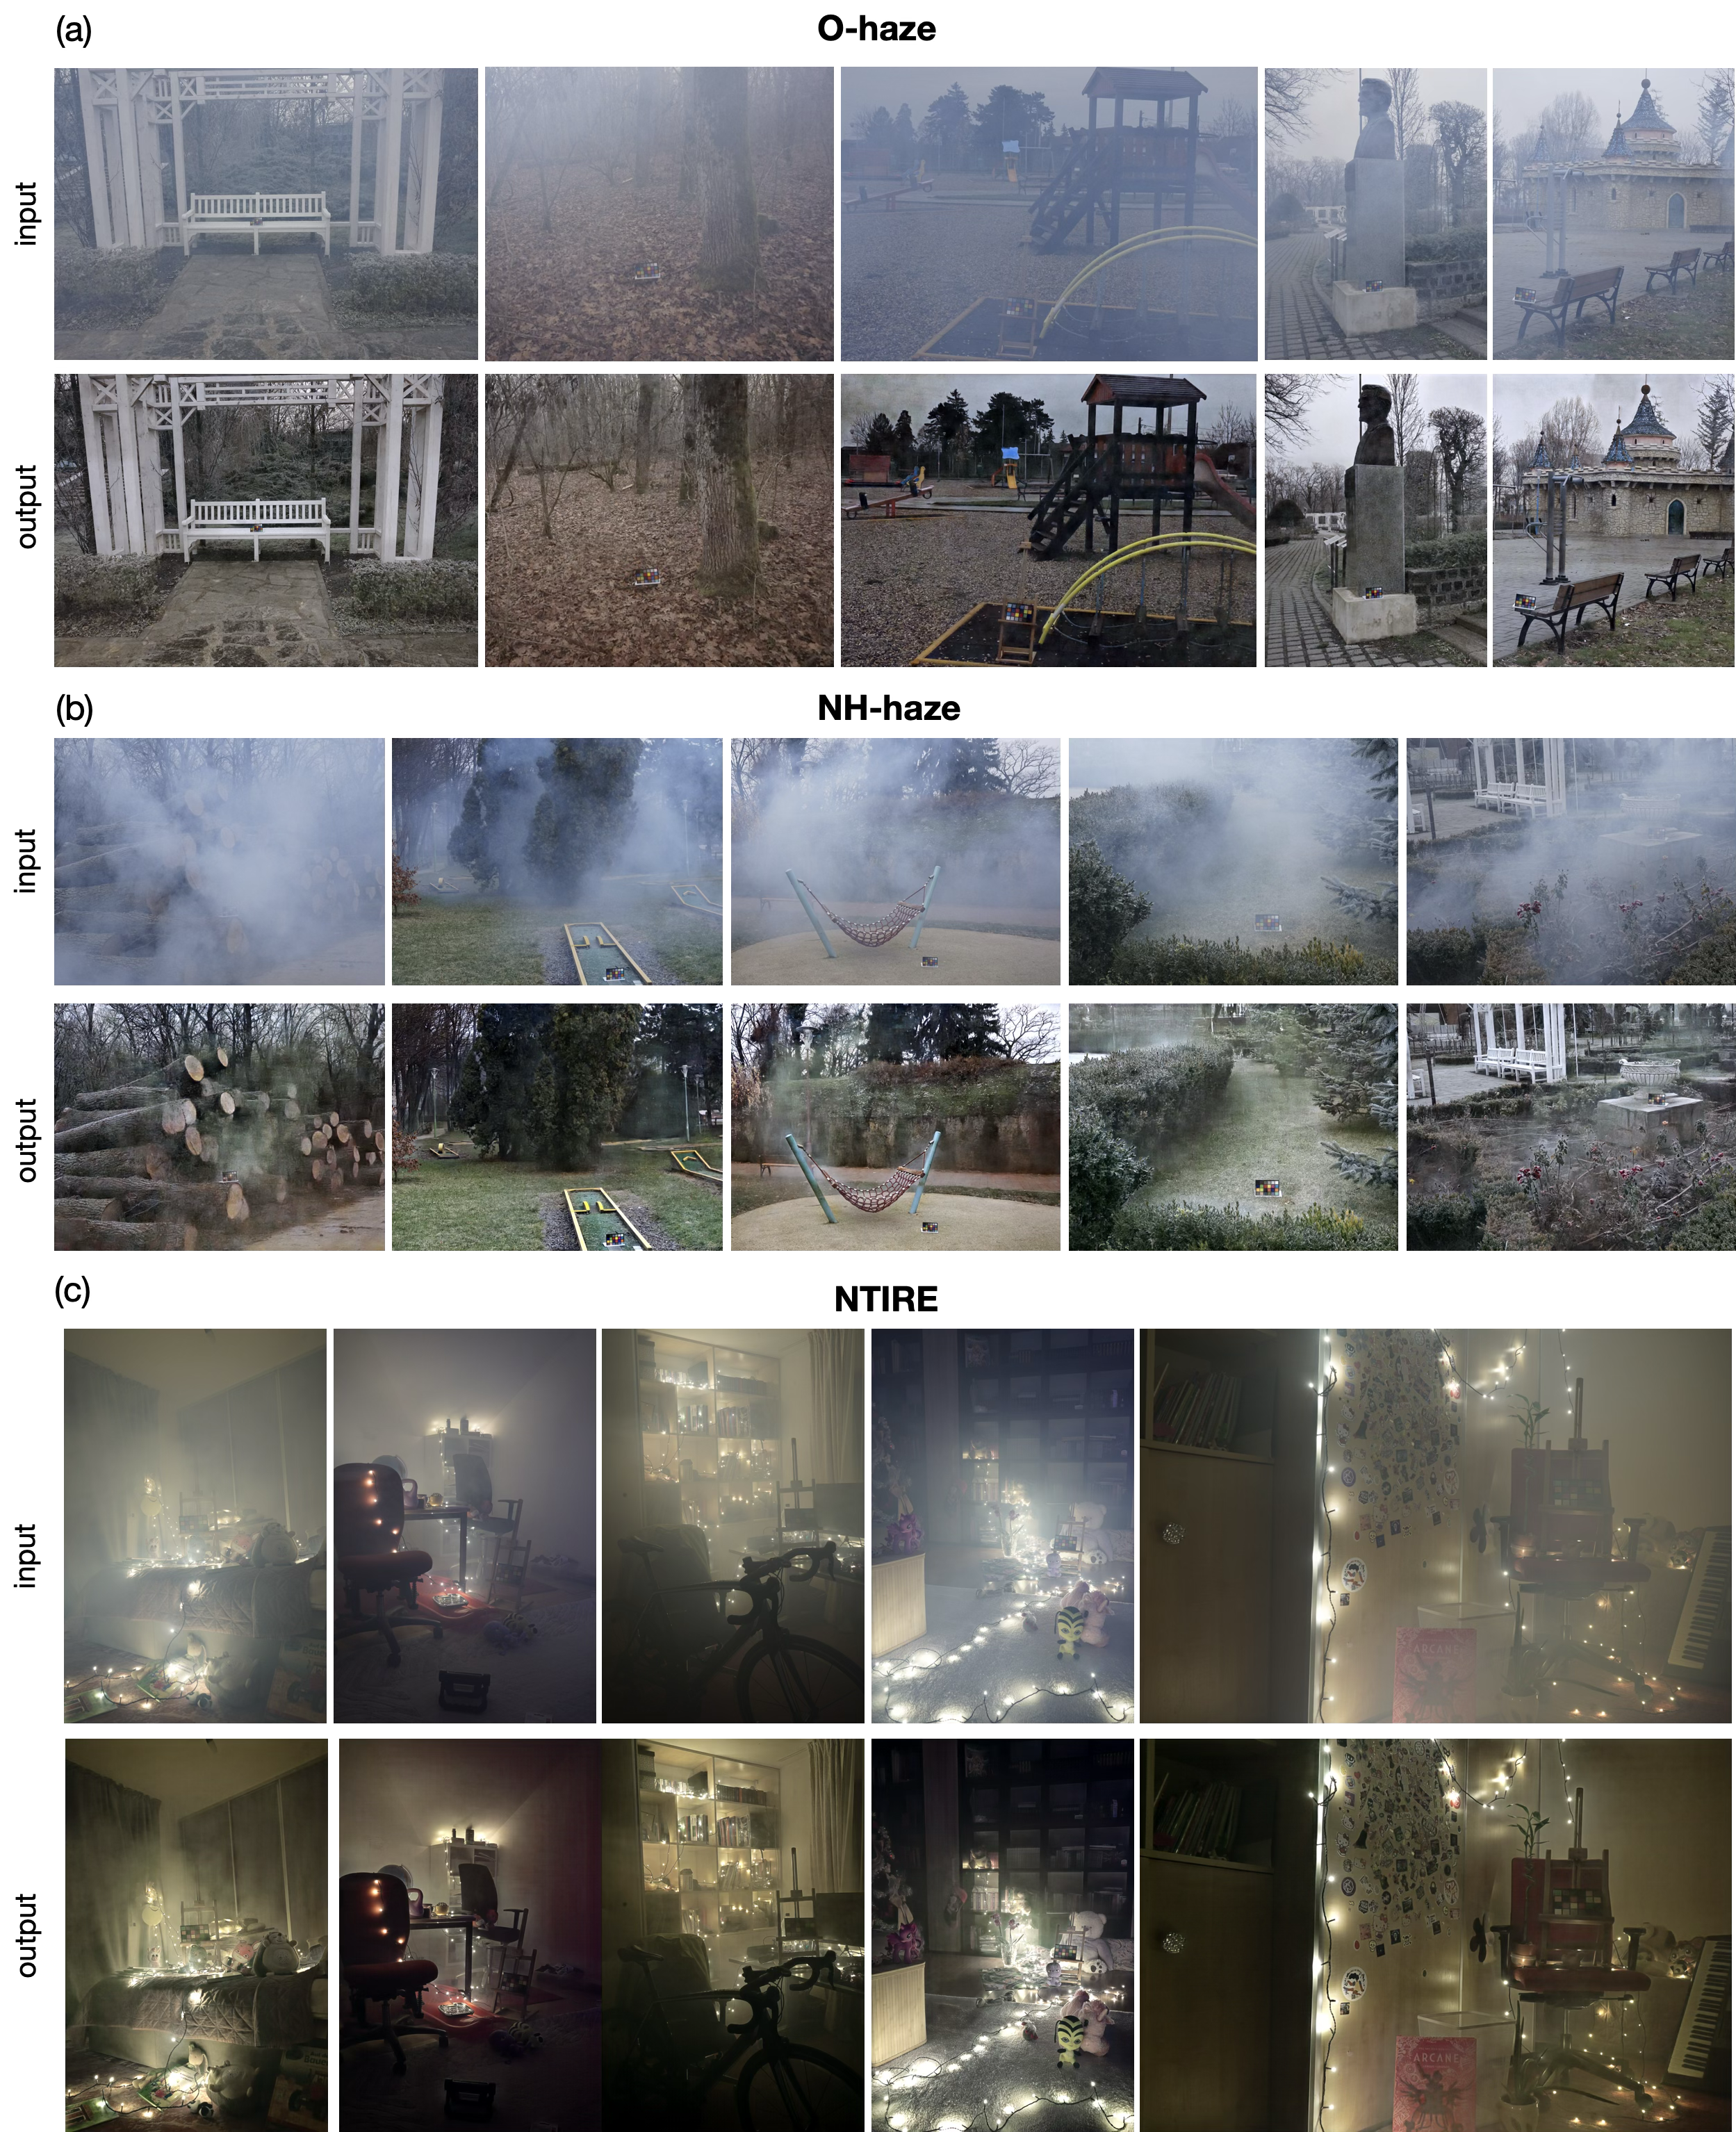
\includegraphics[width=\linewidth]{O-NH_haze_NTIRE.png}
\caption{Task-specific public-haze and nighttime-haze checks. (a) O-HAZE,
(b) NH-HAZE, and (c) NTIRE. Representative images span different haze
severities. The fog-chamber NAFNet was separately fine-tuned on each
paired dataset. Split definitions and metrics are reported in
Supplementary Sections~S7 and~S8.}
\label{fig:O_NH_haze}
\end{figure}
\subsection{Public paired real-haze adaptation}
\label{subsec:realhaze_results}
 
The same backbone adapts under paired supervision. On a
non-overlapping combined split it reached $20.71~\mathrm{dB}$ /
$0.683$~SSIM (O-HAZE subset $22.65$ / $0.726$; NH-HAZE subset
$18.77$ / $0.640$; the $3.88~\mathrm{dB}$ gap reflects
non-homogeneous haze). Exemplary results are summarized in
Fig.~\ref{fig:O_NH_haze}. These are controlled transferability checks,
not competitive claims; dedicated O-HAZE methods exceed
$24~\mathrm{dB}$ \cite{chen2024pttd,chen2025dehazexl}.
Real-fog video with aligned references is the natural next-step
measurement (see Limitations).
An NTIRE 2026 nighttime probe reached $24.77~\mathrm{dB}$ /
$0.770$~SSIM on a two-image internal split (a probe only, no
challenge rank claimed)~\cite{ancuti2026ntire,ancuti2026nt}. Category recognizability and
classification-chain results are in Supplement~S4.

\subsection{Benchmark and paired difficulty metric}
\label{subsec:benchmark_results}
 
NAFNet ranked highest on the 552-image split with mean PSNR
$24.33~\mathrm{dB}$ (95\% bootstrap CI, 24.00--24.65) and SSIM $0.7912$ (95\% bootstrap CI, 0.7808--0.8012), a $12.53~\mathrm{dB}$ gain
over the foggy-input baseline ($11.80~\mathrm{dB}$); SpecAT~S2~\cite{yao2024specat} and
RegGAN followed at $23.04$ and $22.54~\mathrm{dB}$. The parameter-efficiency comparison
(Fig.~\ref{fig:benchmark}) has two anchors: NAFNet
($29.16~\mathrm{M}$ params) for accuracy and SpecAT~S2
($0.99~\mathrm{M}$) for efficiency, the latter within
$1.29~\mathrm{dB}$ at $\approx 3\%$ of the parameters; intermediate models are Pareto-dominated (\emph{i.e.}, worse on both axes than at least one of NAFNet or SpecAT S2). Notably, \texttt{pix2pix}, the adversarial
backbone used for binocular real-world defogging
\cite{isola2017pix2pix, pollak2024stereofog}, ranks low here ($15.58~\mathrm{dB}$):
exact registration favors direct L1 reconstruction over adversarial
translation in this regime. The dark channel prior
\cite{he2010single} reduced PSNR below the foggy input ($11.80
\rightarrow 9.82~\mathrm{dB}$), consistent with the display
back-illumination violating its outdoor assumptions. The full 30-model
table is in Supplementary Table~S2.
 
Per-category PSNR spans $3.42~\mathrm{dB}$ (artwork $23.02$,
furniture $26.44$). Categories with dense fine structure retain less high-frequency
content at a given fog level and are harder to restore
(Supplementary Section~S10).
\begin{figure}[htbp]
\centering
\includegraphics[width=\linewidth]{benchmark.png}
\caption{Defogging benchmark across established models on the fog-chamber dataset. (a) Thirty-model benchmark summary: marker area encodes mean SSIM, the horizontal axis shows parameter count, and the vertical axis shows mean PSNR. (b) Exemplary images from left to right: foggy input, outputs from RegGAN, SpecAT S2, and NAFNet, and ground truth.}
\label{fig:benchmark}
\end{figure}

%% ============================================================
\section{Discussion}
\label{sec:discussion}

The results address a tension in prior real-world defogging.
Pollak and Menon found that models trained on a large real-world
paired dataset transferred poorly across cameras and scenes, and
that generic synthetic fog failed on real
images~\cite{pollak2024stereofog}. Two design choices in the present
work support transfer tests beyond the training apparatus. First,
single-camera display imaging
gives exact pixel registration, which enables pixel-exact
$L_1$ reconstruction and so avoids the adversarial hallucination
that the binocular setting had to tolerate; the same registration
underwrites the paired Laplacian ratio of
Section~\ref{subsec:fogdifficulty}.
Second, a small synthetic stream is interleaved with chamber training
from random initialization, exposing the model throughout
optimization to a broad family of spatially varying outdoor-like
scattering conditions. This arrangement targets oversaturation and
tile-stitching artifacts without imposing a final synthetic-only
stage, while chamber holdout performance remains comparable to the
separately trained architecture-selection model. The two data regimes
are complementary points in a design space: binocular capture trades
registration for real three-dimensional scene content, while display
capture trades scene realism for exact registration and content
control. Together, a carefully posed imaging setup and a
domain-randomized forward model provide complementary supervision
when large-scale paired outdoor collection is impractical.

The aircraft-window evaluation is reference-free (NIQE only) and so
cannot penalize over-correction the way paired PSNR/SSIM can. We
therefore frame the
aircraft-window result as evidence that the pipeline can be applied
framewise on an entirely unseen sensor, scene, and optical path,
rather than as a quantitative generalization or temporal-consistency
claim. Establishing the stronger claim requires aligned
cross-hardware video references, which the present pipeline does not
yet provide.

For practitioners, the benchmark gives two actionable findings.
SpecAT~S2 matches NAFNet within 1.29~dB at roughly 3\% of the
parameters, making it the natural choice when compute or memory is
constrained, and NAFNet is the natural choice when accuracy
dominates. More broadly, exact-registration training favors direct
$L_1$ reconstruction over adversarial translation in this regime,
which inverts the methodological preference reported under
misregistered binocular capture~\cite{pollak2024stereofog}. The
paired Laplacian ratio (Spearman $\rho = 0.632$ versus $0.399$ for
the best single-image proxy) gives a usable per-image difficulty
estimator that, unlike single-image Laplacian variance, is robust
to scene content.

\subsection{Limitations}
\label{sec:limitations}
Five limitations should temper the present claims. (i)~The
fog-chamber capture uses flat display content rather than
three-dimensional scenes, which constrains the realism of training
imagery; the concurrent synthetic stream and the public-haze adaptation
partially, but not fully, compensate. (ii)~The display, camera
response, exposure, and fog radiance were not independently
calibrated, so the chamber data support learned restoration but do
not support radiometric inversion (Section~\ref{sec:fogphysics}).
(iii)~The mixed schedule was evaluated for one primary synthetic
fraction and one completed 5$\times$ sensitivity setting; this does
not establish an optimal mixture, and synthetic scores remain
generator-specific diagnostics. (iv)~The public real-haze and NTIRE
test splits are small, and
the NTIRE 2026 nighttime evaluation is a two-image probe rather
than a competitive ranking. (v)~The aircraft-window evaluation
is reference-free; we report NIQE and demonstration videos, but
PSNR/SSIM-grade evidence of cross-hardware generalization will
require small aligned real-fog video sets. Radiometric calibration
of the apparatus and the collection of such aligned real-fog video
sets are the natural next steps.
 
%% ============================================================
\section{Conclusion}
\label{sec:conclusion}

We presented a controlled display-based fog imager whose exact pixel
registration enables a paired fog-difficulty metric and pixel-exact
reconstruction training. A NAFNet model initialized randomly and trained
on an interleaved mixture of chamber pairs and domain-randomized
synthetic fog reaches comparable chamber holdout performance while
broadening the training distribution. The resulting pipeline is
applied across a
graded sequence of out-of-distribution
settings with no target-domain training: from outdoor captures through
free-flowing fog outside the chamber, in which the optical depth along the
line of sight is no longer fixed by chamber geometry, to iPhone video
recorded through an aircraft cabin window in flight, directly
probing the cross-hardware transfer limitation reported for
real-world binocular defogging~\cite{pollak2024stereofog}. The
aircraft-window evaluation is reference-free, and a small aligned
cross-hardware test set is the natural next measurement.

Supporting evidence comes from four controlled checks. First, NAFNet
leads a uniformly trained 30-model benchmark on the fog-chamber split
at 24.33~dB~/~0.7912~SSIM, with a compact alternative within 1.29~dB
at roughly 3\% of the parameter count, giving practitioners a usable
accuracy--efficiency frontier. Second, a ResNet-50 classifier on
foggy, defogged, and clear inputs shows that the restoration
preserves semantic content rather than only low-level appearance.
Third, the paired Laplacian ratio predicts per-image restoration
difficulty substantially better than single-image proxies
(Spearman $\rho = 0.632$ versus $0.399$), see Supplementary Section~S10. Fourth, the same backbone adapts under paired supervision to O-HAZE/NH-HAZE and to an NTIRE~2026
nighttime probe, showing that the selected architecture remains
trainable outside the chamber domain when paired supervision is
available.

Taken together, the final model combines exact-registration
supervision with concurrent synthetic exposure and was applied
without target-domain retraining to free-flowing outdoor fog and real
aerial video. The release of the dataset, code,
simulator, trained models, and demonstration videos is intended to catalyze further
work on transferable defogging, particularly toward aligned real-fog
video benchmarks that the current literature still lacks.

\begin{backmatter}
\bmsection{Funding} A.I. and R.M. acknowledge funding from US Department of Energy grant \#55801063. S.D.M. and M.Y. acknowledge support through the Science and Engineering Apprenticeship Program (SEAP), administered by the American Society for Engineering Education (ASEE) on behalf of the Office of Naval Research, Department of the Navy. J.D.H. acknowledges support through the Naval Research Enterprise Intern Program (NREAP). 

\bmsection{Acknowledgment} The support and resources from the Center for High Performance Computing at the University of Utah are gratefully acknowledged.

\bmsection{Disclosures} The authors declare no conflicts of interest. The authors used Claude (Anthropic) solely for grammar refinement and organizational suggestions. 

\bmsection{Data Availability} The fog-chamber dataset is available
through Kaggle
\url{https://www.kaggle.com/datasets/alingold/fog-chamber}. Code,
simulator settings, final mixed-data checkpoints, and demonstration
videos underlying this analysis will be released in the project
repository
\url{https://github.com/theMenonlab/defogging} with the
reproducibility package.

\bmsection{Supplemental document}
See Supplement 1 for supporting content including dataset split audits, metric definitions, the full benchmark table, classification and dark-channel-prior checks, joint mixed-data training details, public real-haze protocols, fog-density statistics, PSD analysis, and paired structure-loss analysis.

\end{backmatter}

\bibliography{sample}

\end{document}
